% scratch tex file for trying out stuff for presentation.

% This text is proprietary.
% It's a part of presentation made by myself.
% It may not used commercial.
% The noncommercial use such as private and study is free
% May 2007
% Author: Sascha Frank 
% University Freiburg 
% www.informatik.uni-freiburg.de/~frank/
%
% 
\documentclass{beamer}
\setbeamertemplate{navigation symbols}{}

\usepackage{beamerthemeshadow}
\begin{document}
\title{SiScLab Project 8}  
\author{Katta, Partmann, Wasmer}
\date{\today} 

% \begin{frame}
% \titlepage
% \end{frame}

\section{Implementation}
\label{sec:implementation}


\begin{frame}\frametitle{Module Design}
    TODO \texttt{hdf} preprocessor as self-contained module built for extension
    TODO \texttt{plot} visualization common to all frontends
    TODO \texttt{tk, jupyter} 2 interactive frontends 
\end{frame}



\begin{frame}\frametitle{Visualization Module}
    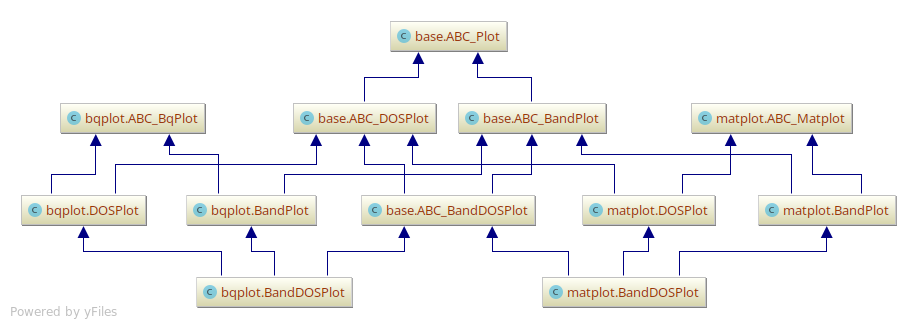
\includegraphics[scale=0.4]{img/pycharm_uml/matplot.png}
\end{frame}

\subsection{Desktop Frontend}
\label{sec:desktop-frontend}

\begin{frame}\frametitle{Desktop Frontend}
    TODO Praneeth?
\end{frame}

\subsection{Web Frontend}
\label{sec:web-frontend}

\begin{frame}\frametitle{Web Frontend}
    TODO Selection Process from Notes 
\end{frame}

\begin{frame}\frametitle{Web Frontend}
    TODO Selection Process Choices from Notes 
\end{frame}





\end{document}



%%% Local Variables:
%%% mode: latex
%%% TeX-master: t
%%% End:
